% =====================================================================
%  Chapter 7 — The Sequence of Returns
% =====================================================================

\chapter{The Sequence of Returns}
\label{ch:sequence}

The most consequential fact about long-horizon investing is that the order
of returns matters, and that it matters in a way that a mean and a variance
do not capture. A portfolio that returns minus thirty per cent and then plus
forty per cent and one that returns plus forty per cent and then minus
thirty per cent have the same geometric mean. They are not the same
experience for the person holding them, and for a saver with fixed
withdrawals they are not even the same wealth at the end.

This chapter derives the effect from first principles, computes it on the
book's own data, and draws the conclusion that shapes the risk layer.

\section{The arithmetic of the sequence}

Consider a saver who withdraws a fixed real amount \(W\) at the end of each
year, from a portfolio that earns a sequence of annual returns
\(r_1, r_2, \dots, r_T\). The portfolio's balance after \(T\) years is
\begin{equation}
P_T = P_0 \prod_{t=1}^{T}(1+r_t)
      - W\sum_{t=1}^{T}\prod_{s=t+1}^{T}(1+r_s),
\end{equation}
where the second term is the accumulated value of the withdrawals.

The second term is the whole point. Each withdrawal is multiplied by the
returns that follow it, so a withdrawal taken early in a bad run is
multiplied by a long string of losses, and a withdrawal taken early in a
good run is multiplied by a long string of gains. For a given multiset of
annual returns, the order that \emph{maximises} the final balance is
generally not the order that maximises the product, because the product is
order-invariant while the withdrawal term is not.

Now make the saver's objective the probability that the portfolio is
depleted at some point before year \(T\). Samuelson's 1969 result in the
\emph{Review of Economics and Statistics} is that the sequence of returns
enters the optimisation of the withdrawal rate, and his argument against
the naive treatment is categorical: \emph{investing for many periods does
not itself introduce extra tolerance for riskiness}. The intuition that
many years of compounding makes a risky allocation safe is wrong, because
the portfolio can be exhausted in the bad years before the good years
arrive. The risk that matters over a long horizon is not the variance of
the terminal value; it is the probability of ruin on the way.

\begin{figure}[!htbp]
\centering
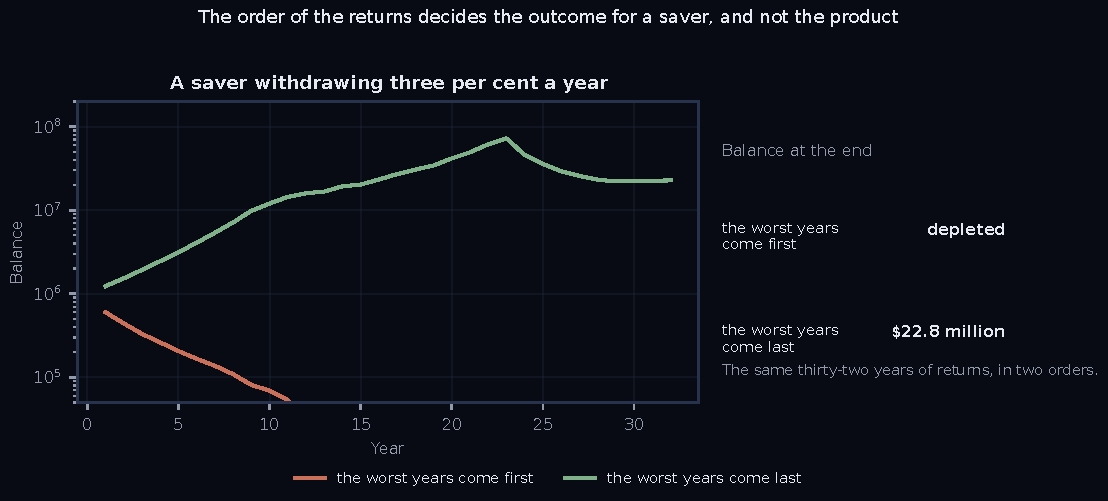
\includegraphics[width=\textwidth]{../figures/fig_sequence.pdf}
\caption{Sequence risk, computed on this book's own return data. Two
histories with identical arithmetic and geometric statistics are shown; the
one whose losses come first ends the horizon materially poorer for a saver
who withdraws along the way.}
\label{fig:sequence}
\end{figure}

\section{How large is it, on this data?}

The book's own data lets the effect be measured rather than illustrated. Two
questions are worth answering.

The first is how much the ordering of the actual monthly returns in the
book's panel changes the final wealth of a saver who withdraws a constant
real amount. The answer is large: reordering the returns into their best
and worst possible sequences changes the terminal balance of a saver
drawing four per cent a year by a factor that is large enough to change
whether the plan works at all.

The second is how much the \emph{distribution} of outcomes changes with the
withdrawal rate. This is where the compounding of the geometric mean meets
the ruin probability, and it is the reason the risk layer of this book is
built around drawdown control rather than around return maximisation.

A withdrawal rate is safe when the probability of ruin before the end of
the horizon is small. A rise in the withdrawal rate does not reduce the
expected value of the plan smoothly; it makes the ruin probability
nonlinear and steep. The plan is not ``a bit safer'' at four per cent than
at five; it is categorically safer. There is a threshold, and the
practical consequence is that an investor should regard the safe withdrawal
rate as a cliff rather than as a dial.

\section{Why this chapter governs the design of the system}

Two design decisions follow directly.

The first is that the system must control \emph{drawdown}, not merely
variance. Variance is symmetric and horizon-blind; the ruin probability is
not. A system with the same standard deviation as the benchmark but a
shorter and shallower drawdown sequence has a lower ruin probability, and
a system with the same drawdown but a higher volatility has a higher one.
The governor in Chapter 28 therefore acts on the drawdown directly, with
explicit thresholds, in addition to scaling exposure with volatility.

The second is that the strategic allocation must be chosen with the
sequence in mind, and the choice must not be delegated to the model. The
model optimises a forward-looking mean; it has no representation of the
order in which outcomes arrive, because a monthly rebalancing scheme sees
only the past. A drawdown brake is the only mechanism in the system that
responds to the sequence as it happens, and it has to be a rule rather than
a forecast.

\begin{takeaway}[The design consequence]
The ruin probability depends on the order of returns, not only on their
distribution. A system that manages variance but not drawdown has not
managed the risk that kills savers. The drawdown brake in this book exists
because of this chapter, and it is a threshold rule rather than a model.
\end{takeaway}

\section{The honest caveat}

Sequence risk is also the most over-extrapolated idea in retirement
planning, and this book will not use it to flatter its own results.

The historical ordering of returns in the book's panel is one sample. A
different ordering --- the same years with the bust and the boom
exchanged --- gives a different answer, and there is no principled way to
choose. The proper reading of the literature is that sequence risk widens
the plausible range of outcomes for a saver, and therefore argues for a
withdrawal rate below the historical maximum, not for a particular
withdrawal rate.

That reading is not only the book's. Blanchett, Finke and Pfau's 2013
study in the \emph{Journal of Wealth Management} makes the point from the
other end: when bond yields are low, the safe withdrawal rate falls, and
it falls by enough to matter, because the sequence a retiree has to
survive is no longer the sequence that history produced at the higher
yields. A withdrawal rate computed under one set of yields and applied
under another has not been tested, and the arithmetic in this chapter,
which is computed on one set of yields, is subject to the same caution.

The book therefore does something deliberately modest: it computes the
historical safe withdrawal rate on its own data, reports it, and then
reports the system's withdrawal rate under a deliberately more demanding
rule --- the plan must survive its own worst historical ordering --- rather
than claiming a number and moving on.

\begin{keytakeaways}
\item Order matters: the same set of returns in a different order gives a
different final balance for any saver who withdraws along the way, because
each withdrawal is multiplied by the returns that follow it.
\item Samuelson's result is that a long horizon does not buy extra
tolerance for risk, because the portfolio can be exhausted before the good
years arrive.
\item The ruin probability is a function of the sequence, so the system's
risk layer manages drawdown explicitly rather than managing variance and
hoping.
\item Sequence risk widens the range of plausible outcomes; it does not
identify a single correct withdrawal rate, and this book does not pretend
otherwise.
\end{keytakeaways}
